% Created by tikzDevice version 0.12.6 on 2025-02-14 09:02:10
% !TEX encoding = UTF-8 Unicode
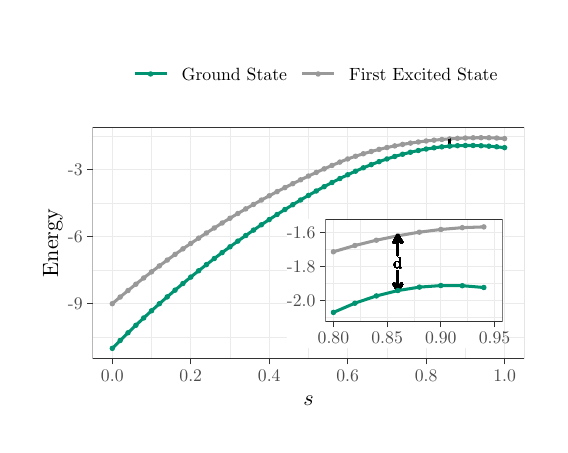
\begin{tikzpicture}[x=1pt,y=1pt]
\definecolor{fillColor}{RGB}{255,255,255}
\path[use as bounding box,fill=fillColor,fill opacity=0.00] (0,0) rectangle (184.92,143.50);
\begin{scope}
\path[clip] (  0.00,  0.00) rectangle (184.92,143.50);
\definecolor{drawColor}{RGB}{255,255,255}
\definecolor{fillColor}{RGB}{255,255,255}

\path[draw=drawColor,line width= 0.6pt,line join=round,line cap=round,fill=fillColor] (  0.00,  0.00) rectangle (184.92,143.50);
\end{scope}
\begin{scope}
\path[clip] (  5.50,  5.50) rectangle (179.42,138.00);
\definecolor{drawColor}{RGB}{255,255,255}
\definecolor{fillColor}{RGB}{255,255,255}

\path[draw=drawColor,line width= 0.4pt,line join=round,line cap=round,fill=fillColor] (  5.50,  5.50) rectangle (179.42,138.00);
\end{scope}
\begin{scope}
\path[clip] ( 23.50, 23.82) rectangle (179.42,107.55);
\definecolor{fillColor}{RGB}{255,255,255}

\path[fill=fillColor] ( 23.50, 23.82) rectangle (179.42,107.55);
\definecolor{drawColor}{gray}{0.92}

\path[draw=drawColor,line width= 0.2pt,line join=round] ( 23.50, 31.66) --
	(179.42, 31.66);

\path[draw=drawColor,line width= 0.2pt,line join=round] ( 23.50, 55.86) --
	(179.42, 55.86);

\path[draw=drawColor,line width= 0.2pt,line join=round] ( 23.50, 80.06) --
	(179.42, 80.06);

\path[draw=drawColor,line width= 0.2pt,line join=round] ( 23.50,104.26) --
	(179.42,104.26);

\path[draw=drawColor,line width= 0.2pt,line join=round] ( 44.76, 23.82) --
	( 44.76,107.55);

\path[draw=drawColor,line width= 0.2pt,line join=round] ( 73.11, 23.82) --
	( 73.11,107.55);

\path[draw=drawColor,line width= 0.2pt,line join=round] (101.46, 23.82) --
	(101.46,107.55);

\path[draw=drawColor,line width= 0.2pt,line join=round] (129.81, 23.82) --
	(129.81,107.55);

\path[draw=drawColor,line width= 0.2pt,line join=round] (158.15, 23.82) --
	(158.15,107.55);

\path[draw=drawColor,line width= 0.4pt,line join=round] ( 23.50, 43.76) --
	(179.42, 43.76);

\path[draw=drawColor,line width= 0.4pt,line join=round] ( 23.50, 67.96) --
	(179.42, 67.96);

\path[draw=drawColor,line width= 0.4pt,line join=round] ( 23.50, 92.16) --
	(179.42, 92.16);

\path[draw=drawColor,line width= 0.4pt,line join=round] ( 30.58, 23.82) --
	( 30.58,107.55);

\path[draw=drawColor,line width= 0.4pt,line join=round] ( 58.93, 23.82) --
	( 58.93,107.55);

\path[draw=drawColor,line width= 0.4pt,line join=round] ( 87.28, 23.82) --
	( 87.28,107.55);

\path[draw=drawColor,line width= 0.4pt,line join=round] (115.63, 23.82) --
	(115.63,107.55);

\path[draw=drawColor,line width= 0.4pt,line join=round] (143.98, 23.82) --
	(143.98,107.55);

\path[draw=drawColor,line width= 0.4pt,line join=round] (172.33, 23.82) --
	(172.33,107.55);
\definecolor{drawColor}{gray}{0.60}

\path[draw=drawColor,line width= 1.1pt,line join=round] ( 30.58, 43.76) --
	( 33.42, 46.16) --
	( 36.25, 48.51) --
	( 39.09, 50.81) --
	( 41.92, 53.06) --
	( 44.76, 55.26) --
	( 47.59, 57.41) --
	( 50.43, 59.52) --
	( 53.26, 61.57) --
	( 56.10, 63.57) --
	( 58.93, 65.53) --
	( 61.77, 67.44) --
	( 64.60, 69.31) --
	( 67.44, 71.13) --
	( 70.27, 72.92) --
	( 73.11, 74.65) --
	( 75.94, 76.35) --
	( 78.78, 78.01) --
	( 81.61, 79.62) --
	( 84.45, 81.20) --
	( 87.28, 82.74) --
	( 90.12, 84.24) --
	( 92.95, 85.71) --
	( 95.79, 87.13) --
	( 98.62, 88.52) --
	(101.46, 89.88) --
	(104.29, 91.20) --
	(107.13, 92.48) --
	(109.96, 93.72) --
	(112.80, 94.92) --
	(115.63, 96.06) --
	(118.47, 97.04) --
	(121.30, 97.94) --
	(124.14, 98.76) --
	(126.97, 99.51) --
	(129.81,100.18) --
	(132.64,100.78) --
	(135.48,101.32) --
	(138.31,101.79) --
	(141.15,102.19) --
	(143.98,102.55) --
	(146.82,102.85) --
	(149.65,103.10) --
	(152.49,103.31) --
	(155.32,103.49) --
	(158.15,103.62) --
	(160.99,103.70) --
	(163.82,103.74) --
	(166.66,103.72) --
	(169.49,103.61) --
	(172.33,103.41);
\definecolor{fillColor}{gray}{0.60}

\path[draw=drawColor,line width= 0.4pt,line join=round,line cap=round,fill=fillColor] ( 30.58, 43.76) circle (  0.78);

\path[draw=drawColor,line width= 0.4pt,line join=round,line cap=round,fill=fillColor] ( 33.42, 46.16) circle (  0.78);

\path[draw=drawColor,line width= 0.4pt,line join=round,line cap=round,fill=fillColor] ( 36.25, 48.51) circle (  0.78);

\path[draw=drawColor,line width= 0.4pt,line join=round,line cap=round,fill=fillColor] ( 39.09, 50.81) circle (  0.78);

\path[draw=drawColor,line width= 0.4pt,line join=round,line cap=round,fill=fillColor] ( 41.92, 53.06) circle (  0.78);

\path[draw=drawColor,line width= 0.4pt,line join=round,line cap=round,fill=fillColor] ( 44.76, 55.26) circle (  0.78);

\path[draw=drawColor,line width= 0.4pt,line join=round,line cap=round,fill=fillColor] ( 47.59, 57.41) circle (  0.78);

\path[draw=drawColor,line width= 0.4pt,line join=round,line cap=round,fill=fillColor] ( 50.43, 59.52) circle (  0.78);

\path[draw=drawColor,line width= 0.4pt,line join=round,line cap=round,fill=fillColor] ( 53.26, 61.57) circle (  0.78);

\path[draw=drawColor,line width= 0.4pt,line join=round,line cap=round,fill=fillColor] ( 56.10, 63.57) circle (  0.78);

\path[draw=drawColor,line width= 0.4pt,line join=round,line cap=round,fill=fillColor] ( 58.93, 65.53) circle (  0.78);

\path[draw=drawColor,line width= 0.4pt,line join=round,line cap=round,fill=fillColor] ( 61.77, 67.44) circle (  0.78);

\path[draw=drawColor,line width= 0.4pt,line join=round,line cap=round,fill=fillColor] ( 64.60, 69.31) circle (  0.78);

\path[draw=drawColor,line width= 0.4pt,line join=round,line cap=round,fill=fillColor] ( 67.44, 71.13) circle (  0.78);

\path[draw=drawColor,line width= 0.4pt,line join=round,line cap=round,fill=fillColor] ( 70.27, 72.92) circle (  0.78);

\path[draw=drawColor,line width= 0.4pt,line join=round,line cap=round,fill=fillColor] ( 73.11, 74.65) circle (  0.78);

\path[draw=drawColor,line width= 0.4pt,line join=round,line cap=round,fill=fillColor] ( 75.94, 76.35) circle (  0.78);

\path[draw=drawColor,line width= 0.4pt,line join=round,line cap=round,fill=fillColor] ( 78.78, 78.01) circle (  0.78);

\path[draw=drawColor,line width= 0.4pt,line join=round,line cap=round,fill=fillColor] ( 81.61, 79.62) circle (  0.78);

\path[draw=drawColor,line width= 0.4pt,line join=round,line cap=round,fill=fillColor] ( 84.45, 81.20) circle (  0.78);

\path[draw=drawColor,line width= 0.4pt,line join=round,line cap=round,fill=fillColor] ( 87.28, 82.74) circle (  0.78);

\path[draw=drawColor,line width= 0.4pt,line join=round,line cap=round,fill=fillColor] ( 90.12, 84.24) circle (  0.78);

\path[draw=drawColor,line width= 0.4pt,line join=round,line cap=round,fill=fillColor] ( 92.95, 85.71) circle (  0.78);

\path[draw=drawColor,line width= 0.4pt,line join=round,line cap=round,fill=fillColor] ( 95.79, 87.13) circle (  0.78);

\path[draw=drawColor,line width= 0.4pt,line join=round,line cap=round,fill=fillColor] ( 98.62, 88.52) circle (  0.78);

\path[draw=drawColor,line width= 0.4pt,line join=round,line cap=round,fill=fillColor] (101.46, 89.88) circle (  0.78);

\path[draw=drawColor,line width= 0.4pt,line join=round,line cap=round,fill=fillColor] (104.29, 91.20) circle (  0.78);

\path[draw=drawColor,line width= 0.4pt,line join=round,line cap=round,fill=fillColor] (107.13, 92.48) circle (  0.78);

\path[draw=drawColor,line width= 0.4pt,line join=round,line cap=round,fill=fillColor] (109.96, 93.72) circle (  0.78);

\path[draw=drawColor,line width= 0.4pt,line join=round,line cap=round,fill=fillColor] (112.80, 94.92) circle (  0.78);

\path[draw=drawColor,line width= 0.4pt,line join=round,line cap=round,fill=fillColor] (115.63, 96.06) circle (  0.78);

\path[draw=drawColor,line width= 0.4pt,line join=round,line cap=round,fill=fillColor] (118.47, 97.04) circle (  0.78);

\path[draw=drawColor,line width= 0.4pt,line join=round,line cap=round,fill=fillColor] (121.30, 97.94) circle (  0.78);

\path[draw=drawColor,line width= 0.4pt,line join=round,line cap=round,fill=fillColor] (124.14, 98.76) circle (  0.78);

\path[draw=drawColor,line width= 0.4pt,line join=round,line cap=round,fill=fillColor] (126.97, 99.51) circle (  0.78);

\path[draw=drawColor,line width= 0.4pt,line join=round,line cap=round,fill=fillColor] (129.81,100.18) circle (  0.78);

\path[draw=drawColor,line width= 0.4pt,line join=round,line cap=round,fill=fillColor] (132.64,100.78) circle (  0.78);

\path[draw=drawColor,line width= 0.4pt,line join=round,line cap=round,fill=fillColor] (135.48,101.32) circle (  0.78);

\path[draw=drawColor,line width= 0.4pt,line join=round,line cap=round,fill=fillColor] (138.31,101.79) circle (  0.78);

\path[draw=drawColor,line width= 0.4pt,line join=round,line cap=round,fill=fillColor] (141.15,102.19) circle (  0.78);

\path[draw=drawColor,line width= 0.4pt,line join=round,line cap=round,fill=fillColor] (143.98,102.55) circle (  0.78);

\path[draw=drawColor,line width= 0.4pt,line join=round,line cap=round,fill=fillColor] (146.82,102.85) circle (  0.78);

\path[draw=drawColor,line width= 0.4pt,line join=round,line cap=round,fill=fillColor] (149.65,103.10) circle (  0.78);

\path[draw=drawColor,line width= 0.4pt,line join=round,line cap=round,fill=fillColor] (152.49,103.31) circle (  0.78);

\path[draw=drawColor,line width= 0.4pt,line join=round,line cap=round,fill=fillColor] (155.32,103.49) circle (  0.78);

\path[draw=drawColor,line width= 0.4pt,line join=round,line cap=round,fill=fillColor] (158.15,103.62) circle (  0.78);

\path[draw=drawColor,line width= 0.4pt,line join=round,line cap=round,fill=fillColor] (160.99,103.70) circle (  0.78);

\path[draw=drawColor,line width= 0.4pt,line join=round,line cap=round,fill=fillColor] (163.82,103.74) circle (  0.78);

\path[draw=drawColor,line width= 0.4pt,line join=round,line cap=round,fill=fillColor] (166.66,103.72) circle (  0.78);

\path[draw=drawColor,line width= 0.4pt,line join=round,line cap=round,fill=fillColor] (169.49,103.61) circle (  0.78);

\path[draw=drawColor,line width= 0.4pt,line join=round,line cap=round,fill=fillColor] (172.33,103.41) circle (  0.78);
\definecolor{drawColor}{RGB}{0,0,0}

\path[draw=drawColor,line width= 1.1pt,line join=round] (152.49,103.31) -- (152.49,100.69);

\path[draw=drawColor,line width= 1.1pt,line join=round] (152.49,103.31) -- (152.49,100.69);

\path[draw=drawColor,line width= 1.1pt,line join=round] (152.49,103.31) -- (152.49,100.69);

\path[draw=drawColor,line width= 1.1pt,line join=round] (152.49,103.31) -- (152.49,100.69);

\path[draw=drawColor,line width= 1.1pt,line join=round] (152.49,103.31) -- (152.49,100.69);

\path[draw=drawColor,line width= 1.1pt,line join=round] (152.49,103.31) -- (152.49,100.69);

\path[draw=drawColor,line width= 1.1pt,line join=round] (152.49,103.31) -- (152.49,100.69);

\path[draw=drawColor,line width= 1.1pt,line join=round] (152.49,103.31) -- (152.49,100.69);

\path[draw=drawColor,line width= 1.1pt,line join=round] (152.49,103.31) -- (152.49,100.69);

\path[draw=drawColor,line width= 1.1pt,line join=round] (152.49,103.31) -- (152.49,100.69);

\path[draw=drawColor,line width= 1.1pt,line join=round] (152.49,103.31) -- (152.49,100.69);

\path[draw=drawColor,line width= 1.1pt,line join=round] (152.49,103.31) -- (152.49,100.69);

\path[draw=drawColor,line width= 1.1pt,line join=round] (152.49,103.31) -- (152.49,100.69);

\path[draw=drawColor,line width= 1.1pt,line join=round] (152.49,103.31) -- (152.49,100.69);

\path[draw=drawColor,line width= 1.1pt,line join=round] (152.49,103.31) -- (152.49,100.69);

\path[draw=drawColor,line width= 1.1pt,line join=round] (152.49,103.31) -- (152.49,100.69);

\path[draw=drawColor,line width= 1.1pt,line join=round] (152.49,103.31) -- (152.49,100.69);

\path[draw=drawColor,line width= 1.1pt,line join=round] (152.49,103.31) -- (152.49,100.69);

\path[draw=drawColor,line width= 1.1pt,line join=round] (152.49,103.31) -- (152.49,100.69);

\path[draw=drawColor,line width= 1.1pt,line join=round] (152.49,103.31) -- (152.49,100.69);

\path[draw=drawColor,line width= 1.1pt,line join=round] (152.49,103.31) -- (152.49,100.69);

\path[draw=drawColor,line width= 1.1pt,line join=round] (152.49,103.31) -- (152.49,100.69);

\path[draw=drawColor,line width= 1.1pt,line join=round] (152.49,103.31) -- (152.49,100.69);

\path[draw=drawColor,line width= 1.1pt,line join=round] (152.49,103.31) -- (152.49,100.69);

\path[draw=drawColor,line width= 1.1pt,line join=round] (152.49,103.31) -- (152.49,100.69);

\path[draw=drawColor,line width= 1.1pt,line join=round] (152.49,103.31) -- (152.49,100.69);

\path[draw=drawColor,line width= 1.1pt,line join=round] (152.49,103.31) -- (152.49,100.69);

\path[draw=drawColor,line width= 1.1pt,line join=round] (152.49,103.31) -- (152.49,100.69);

\path[draw=drawColor,line width= 1.1pt,line join=round] (152.49,103.31) -- (152.49,100.69);

\path[draw=drawColor,line width= 1.1pt,line join=round] (152.49,103.31) -- (152.49,100.69);

\path[draw=drawColor,line width= 1.1pt,line join=round] (152.49,103.31) -- (152.49,100.69);

\path[draw=drawColor,line width= 1.1pt,line join=round] (152.49,103.31) -- (152.49,100.69);

\path[draw=drawColor,line width= 1.1pt,line join=round] (152.49,103.31) -- (152.49,100.69);

\path[draw=drawColor,line width= 1.1pt,line join=round] (152.49,103.31) -- (152.49,100.69);

\path[draw=drawColor,line width= 1.1pt,line join=round] (152.49,103.31) -- (152.49,100.69);

\path[draw=drawColor,line width= 1.1pt,line join=round] (152.49,103.31) -- (152.49,100.69);

\path[draw=drawColor,line width= 1.1pt,line join=round] (152.49,103.31) -- (152.49,100.69);

\path[draw=drawColor,line width= 1.1pt,line join=round] (152.49,103.31) -- (152.49,100.69);

\path[draw=drawColor,line width= 1.1pt,line join=round] (152.49,103.31) -- (152.49,100.69);

\path[draw=drawColor,line width= 1.1pt,line join=round] (152.49,103.31) -- (152.49,100.69);

\path[draw=drawColor,line width= 1.1pt,line join=round] (152.49,103.31) -- (152.49,100.69);

\path[draw=drawColor,line width= 1.1pt,line join=round] (152.49,103.31) -- (152.49,100.69);

\path[draw=drawColor,line width= 1.1pt,line join=round] (152.49,103.31) -- (152.49,100.69);

\path[draw=drawColor,line width= 1.1pt,line join=round] (152.49,103.31) -- (152.49,100.69);

\path[draw=drawColor,line width= 1.1pt,line join=round] (152.49,103.31) -- (152.49,100.69);

\path[draw=drawColor,line width= 1.1pt,line join=round] (152.49,103.31) -- (152.49,100.69);

\path[draw=drawColor,line width= 1.1pt,line join=round] (152.49,103.31) -- (152.49,100.69);

\path[draw=drawColor,line width= 1.1pt,line join=round] (152.49,103.31) -- (152.49,100.69);

\path[draw=drawColor,line width= 1.1pt,line join=round] (152.49,103.31) -- (152.49,100.69);

\path[draw=drawColor,line width= 1.1pt,line join=round] (152.49,103.31) -- (152.49,100.69);

\path[draw=drawColor,line width= 1.1pt,line join=round] (152.49,103.31) -- (152.49,100.69);
\definecolor{drawColor}{RGB}{0,147,113}

\path[draw=drawColor,line width= 1.1pt,line join=round] ( 30.58, 27.62) --
	( 33.42, 30.46) --
	( 36.25, 33.24) --
	( 39.09, 35.95) --
	( 41.92, 38.61) --
	( 44.76, 41.20) --
	( 47.59, 43.74) --
	( 50.43, 46.23) --
	( 53.26, 48.66) --
	( 56.10, 51.04) --
	( 58.93, 53.37) --
	( 61.77, 55.65) --
	( 64.60, 57.89) --
	( 67.44, 60.07) --
	( 70.27, 62.22) --
	( 73.11, 64.31) --
	( 75.94, 66.37) --
	( 78.78, 68.38) --
	( 81.61, 70.35) --
	( 84.45, 72.27) --
	( 87.28, 74.15) --
	( 90.12, 75.99) --
	( 92.95, 77.79) --
	( 95.79, 79.53) --
	( 98.62, 81.24) --
	(101.46, 82.89) --
	(104.29, 84.49) --
	(107.13, 86.04) --
	(109.96, 87.54) --
	(112.80, 88.97) --
	(115.63, 90.34) --
	(118.47, 91.64) --
	(121.30, 92.86) --
	(124.14, 94.01) --
	(126.97, 95.08) --
	(129.81, 96.06) --
	(132.64, 96.96) --
	(135.48, 97.76) --
	(138.31, 98.48) --
	(141.15, 99.11) --
	(143.98, 99.64) --
	(146.82,100.08) --
	(149.65,100.43) --
	(152.49,100.69) --
	(155.32,100.85) --
	(158.15,100.93) --
	(160.99,100.92) --
	(163.82,100.83) --
	(166.66,100.68) --
	(169.49,100.45) --
	(172.33,100.15);
\definecolor{fillColor}{RGB}{0,147,113}

\path[draw=drawColor,line width= 0.4pt,line join=round,line cap=round,fill=fillColor] ( 30.58, 27.62) circle (  0.78);

\path[draw=drawColor,line width= 0.4pt,line join=round,line cap=round,fill=fillColor] ( 33.42, 30.46) circle (  0.78);

\path[draw=drawColor,line width= 0.4pt,line join=round,line cap=round,fill=fillColor] ( 36.25, 33.24) circle (  0.78);

\path[draw=drawColor,line width= 0.4pt,line join=round,line cap=round,fill=fillColor] ( 39.09, 35.95) circle (  0.78);

\path[draw=drawColor,line width= 0.4pt,line join=round,line cap=round,fill=fillColor] ( 41.92, 38.61) circle (  0.78);

\path[draw=drawColor,line width= 0.4pt,line join=round,line cap=round,fill=fillColor] ( 44.76, 41.20) circle (  0.78);

\path[draw=drawColor,line width= 0.4pt,line join=round,line cap=round,fill=fillColor] ( 47.59, 43.74) circle (  0.78);

\path[draw=drawColor,line width= 0.4pt,line join=round,line cap=round,fill=fillColor] ( 50.43, 46.23) circle (  0.78);

\path[draw=drawColor,line width= 0.4pt,line join=round,line cap=round,fill=fillColor] ( 53.26, 48.66) circle (  0.78);

\path[draw=drawColor,line width= 0.4pt,line join=round,line cap=round,fill=fillColor] ( 56.10, 51.04) circle (  0.78);

\path[draw=drawColor,line width= 0.4pt,line join=round,line cap=round,fill=fillColor] ( 58.93, 53.37) circle (  0.78);

\path[draw=drawColor,line width= 0.4pt,line join=round,line cap=round,fill=fillColor] ( 61.77, 55.65) circle (  0.78);

\path[draw=drawColor,line width= 0.4pt,line join=round,line cap=round,fill=fillColor] ( 64.60, 57.89) circle (  0.78);

\path[draw=drawColor,line width= 0.4pt,line join=round,line cap=round,fill=fillColor] ( 67.44, 60.07) circle (  0.78);

\path[draw=drawColor,line width= 0.4pt,line join=round,line cap=round,fill=fillColor] ( 70.27, 62.22) circle (  0.78);

\path[draw=drawColor,line width= 0.4pt,line join=round,line cap=round,fill=fillColor] ( 73.11, 64.31) circle (  0.78);

\path[draw=drawColor,line width= 0.4pt,line join=round,line cap=round,fill=fillColor] ( 75.94, 66.37) circle (  0.78);

\path[draw=drawColor,line width= 0.4pt,line join=round,line cap=round,fill=fillColor] ( 78.78, 68.38) circle (  0.78);

\path[draw=drawColor,line width= 0.4pt,line join=round,line cap=round,fill=fillColor] ( 81.61, 70.35) circle (  0.78);

\path[draw=drawColor,line width= 0.4pt,line join=round,line cap=round,fill=fillColor] ( 84.45, 72.27) circle (  0.78);

\path[draw=drawColor,line width= 0.4pt,line join=round,line cap=round,fill=fillColor] ( 87.28, 74.15) circle (  0.78);

\path[draw=drawColor,line width= 0.4pt,line join=round,line cap=round,fill=fillColor] ( 90.12, 75.99) circle (  0.78);

\path[draw=drawColor,line width= 0.4pt,line join=round,line cap=round,fill=fillColor] ( 92.95, 77.79) circle (  0.78);

\path[draw=drawColor,line width= 0.4pt,line join=round,line cap=round,fill=fillColor] ( 95.79, 79.53) circle (  0.78);

\path[draw=drawColor,line width= 0.4pt,line join=round,line cap=round,fill=fillColor] ( 98.62, 81.24) circle (  0.78);

\path[draw=drawColor,line width= 0.4pt,line join=round,line cap=round,fill=fillColor] (101.46, 82.89) circle (  0.78);

\path[draw=drawColor,line width= 0.4pt,line join=round,line cap=round,fill=fillColor] (104.29, 84.49) circle (  0.78);

\path[draw=drawColor,line width= 0.4pt,line join=round,line cap=round,fill=fillColor] (107.13, 86.04) circle (  0.78);

\path[draw=drawColor,line width= 0.4pt,line join=round,line cap=round,fill=fillColor] (109.96, 87.54) circle (  0.78);

\path[draw=drawColor,line width= 0.4pt,line join=round,line cap=round,fill=fillColor] (112.80, 88.97) circle (  0.78);

\path[draw=drawColor,line width= 0.4pt,line join=round,line cap=round,fill=fillColor] (115.63, 90.34) circle (  0.78);

\path[draw=drawColor,line width= 0.4pt,line join=round,line cap=round,fill=fillColor] (118.47, 91.64) circle (  0.78);

\path[draw=drawColor,line width= 0.4pt,line join=round,line cap=round,fill=fillColor] (121.30, 92.86) circle (  0.78);

\path[draw=drawColor,line width= 0.4pt,line join=round,line cap=round,fill=fillColor] (124.14, 94.01) circle (  0.78);

\path[draw=drawColor,line width= 0.4pt,line join=round,line cap=round,fill=fillColor] (126.97, 95.08) circle (  0.78);

\path[draw=drawColor,line width= 0.4pt,line join=round,line cap=round,fill=fillColor] (129.81, 96.06) circle (  0.78);

\path[draw=drawColor,line width= 0.4pt,line join=round,line cap=round,fill=fillColor] (132.64, 96.96) circle (  0.78);

\path[draw=drawColor,line width= 0.4pt,line join=round,line cap=round,fill=fillColor] (135.48, 97.76) circle (  0.78);

\path[draw=drawColor,line width= 0.4pt,line join=round,line cap=round,fill=fillColor] (138.31, 98.48) circle (  0.78);

\path[draw=drawColor,line width= 0.4pt,line join=round,line cap=round,fill=fillColor] (141.15, 99.11) circle (  0.78);

\path[draw=drawColor,line width= 0.4pt,line join=round,line cap=round,fill=fillColor] (143.98, 99.64) circle (  0.78);

\path[draw=drawColor,line width= 0.4pt,line join=round,line cap=round,fill=fillColor] (146.82,100.08) circle (  0.78);

\path[draw=drawColor,line width= 0.4pt,line join=round,line cap=round,fill=fillColor] (149.65,100.43) circle (  0.78);

\path[draw=drawColor,line width= 0.4pt,line join=round,line cap=round,fill=fillColor] (152.49,100.69) circle (  0.78);

\path[draw=drawColor,line width= 0.4pt,line join=round,line cap=round,fill=fillColor] (155.32,100.85) circle (  0.78);

\path[draw=drawColor,line width= 0.4pt,line join=round,line cap=round,fill=fillColor] (158.15,100.93) circle (  0.78);

\path[draw=drawColor,line width= 0.4pt,line join=round,line cap=round,fill=fillColor] (160.99,100.92) circle (  0.78);

\path[draw=drawColor,line width= 0.4pt,line join=round,line cap=round,fill=fillColor] (163.82,100.83) circle (  0.78);

\path[draw=drawColor,line width= 0.4pt,line join=round,line cap=round,fill=fillColor] (166.66,100.68) circle (  0.78);

\path[draw=drawColor,line width= 0.4pt,line join=round,line cap=round,fill=fillColor] (169.49,100.45) circle (  0.78);

\path[draw=drawColor,line width= 0.4pt,line join=round,line cap=round,fill=fillColor] (172.33,100.15) circle (  0.78);
\definecolor{drawColor}{gray}{0.20}

\path[draw=drawColor,line width= 0.4pt,line join=round,line cap=round] ( 23.50, 23.82) rectangle (179.42,107.55);
\end{scope}
\begin{scope}
\path[clip] (  0.00,  0.00) rectangle (184.92,143.50);
\definecolor{drawColor}{gray}{0.30}

\node[text=drawColor,anchor=base east,inner sep=0pt, outer sep=0pt, scale=  0.64] at ( 19.90, 41.55) {-9};

\node[text=drawColor,anchor=base east,inner sep=0pt, outer sep=0pt, scale=  0.64] at ( 19.90, 65.75) {-6};

\node[text=drawColor,anchor=base east,inner sep=0pt, outer sep=0pt, scale=  0.64] at ( 19.90, 89.95) {-3};
\end{scope}
\begin{scope}
\path[clip] (  0.00,  0.00) rectangle (184.92,143.50);
\definecolor{drawColor}{gray}{0.20}

\path[draw=drawColor,line width= 0.4pt,line join=round] ( 21.50, 43.76) --
	( 23.50, 43.76);

\path[draw=drawColor,line width= 0.4pt,line join=round] ( 21.50, 67.96) --
	( 23.50, 67.96);

\path[draw=drawColor,line width= 0.4pt,line join=round] ( 21.50, 92.16) --
	( 23.50, 92.16);
\end{scope}
\begin{scope}
\path[clip] (  0.00,  0.00) rectangle (184.92,143.50);
\definecolor{drawColor}{gray}{0.20}

\path[draw=drawColor,line width= 0.4pt,line join=round] ( 30.58, 21.82) --
	( 30.58, 23.82);

\path[draw=drawColor,line width= 0.4pt,line join=round] ( 58.93, 21.82) --
	( 58.93, 23.82);

\path[draw=drawColor,line width= 0.4pt,line join=round] ( 87.28, 21.82) --
	( 87.28, 23.82);

\path[draw=drawColor,line width= 0.4pt,line join=round] (115.63, 21.82) --
	(115.63, 23.82);

\path[draw=drawColor,line width= 0.4pt,line join=round] (143.98, 21.82) --
	(143.98, 23.82);

\path[draw=drawColor,line width= 0.4pt,line join=round] (172.33, 21.82) --
	(172.33, 23.82);
\end{scope}
\begin{scope}
\path[clip] (  0.00,  0.00) rectangle (184.92,143.50);
\definecolor{drawColor}{gray}{0.30}

\node[text=drawColor,anchor=base,inner sep=0pt, outer sep=0pt, scale=  0.64] at ( 30.58, 15.81) {0.0};

\node[text=drawColor,anchor=base,inner sep=0pt, outer sep=0pt, scale=  0.64] at ( 58.93, 15.81) {0.2};

\node[text=drawColor,anchor=base,inner sep=0pt, outer sep=0pt, scale=  0.64] at ( 87.28, 15.81) {0.4};

\node[text=drawColor,anchor=base,inner sep=0pt, outer sep=0pt, scale=  0.64] at (115.63, 15.81) {0.6};

\node[text=drawColor,anchor=base,inner sep=0pt, outer sep=0pt, scale=  0.64] at (143.98, 15.81) {0.8};

\node[text=drawColor,anchor=base,inner sep=0pt, outer sep=0pt, scale=  0.64] at (172.33, 15.81) {1.0};
\end{scope}
\begin{scope}
\path[clip] (  0.00,  0.00) rectangle (184.92,143.50);
\definecolor{drawColor}{RGB}{0,0,0}

\node[text=drawColor,anchor=base,inner sep=0pt, outer sep=0pt, scale=  0.80] at (101.46,  7.06) {$s$};
\end{scope}
\begin{scope}
\path[clip] (  0.00,  0.00) rectangle (184.92,143.50);
\definecolor{drawColor}{RGB}{0,0,0}

\node[text=drawColor,rotate= 90.00,anchor=base,inner sep=0pt, outer sep=0pt, scale=  0.80] at ( 11.01, 65.68) {Energy};
\end{scope}
\begin{scope}
\path[clip] (  0.00,  0.00) rectangle (184.92,143.50);
\definecolor{fillColor}{RGB}{255,255,255}

\path[fill=fillColor] ( 29.18,115.55) rectangle (173.74,138.00);
\end{scope}
\begin{scope}
\path[clip] (  0.00,  0.00) rectangle (184.92,143.50);
\definecolor{fillColor}{RGB}{255,255,255}

\path[fill=fillColor] ( 37.18,119.55) rectangle ( 51.63,134.00);
\end{scope}
\begin{scope}
\path[clip] (  0.00,  0.00) rectangle (184.92,143.50);
\definecolor{drawColor}{RGB}{0,147,113}

\path[draw=drawColor,line width= 1.1pt,line join=round] ( 38.62,126.77) -- ( 50.19,126.77);
\end{scope}
\begin{scope}
\path[clip] (  0.00,  0.00) rectangle (184.92,143.50);
\definecolor{drawColor}{RGB}{0,147,113}
\definecolor{fillColor}{RGB}{0,147,113}

\path[draw=drawColor,line width= 0.4pt,line join=round,line cap=round,fill=fillColor] ( 44.41,126.77) circle (  0.78);
\end{scope}
\begin{scope}
\path[clip] (  0.00,  0.00) rectangle (184.92,143.50);
\definecolor{fillColor}{RGB}{255,255,255}

\path[fill=fillColor] ( 97.73,119.55) rectangle (112.18,134.00);
\end{scope}
\begin{scope}
\path[clip] (  0.00,  0.00) rectangle (184.92,143.50);
\definecolor{drawColor}{gray}{0.60}

\path[draw=drawColor,line width= 1.1pt,line join=round] ( 99.18,126.77) -- (110.74,126.77);
\end{scope}
\begin{scope}
\path[clip] (  0.00,  0.00) rectangle (184.92,143.50);
\definecolor{drawColor}{gray}{0.60}
\definecolor{fillColor}{gray}{0.60}

\path[draw=drawColor,line width= 0.4pt,line join=round,line cap=round,fill=fillColor] (104.96,126.77) circle (  0.78);
\end{scope}
\begin{scope}
\path[clip] (  0.00,  0.00) rectangle (184.92,143.50);
\definecolor{drawColor}{RGB}{0,0,0}

\node[text=drawColor,anchor=base west,inner sep=0pt, outer sep=0pt, scale=  0.64] at ( 55.63,124.57) {Ground State};
\end{scope}
\begin{scope}
\path[clip] (  0.00,  0.00) rectangle (184.92,143.50);
\definecolor{drawColor}{RGB}{0,0,0}

\node[text=drawColor,anchor=base west,inner sep=0pt, outer sep=0pt, scale=  0.64] at (116.18,124.57) {First Excited State};
\end{scope}
\begin{scope}
\path[clip] ( 93.66, 28.00) rectangle (171.62, 74.05);
\definecolor{drawColor}{RGB}{255,255,255}
\definecolor{fillColor}{RGB}{255,255,255}

\path[draw=drawColor,line width= 0.4pt,line join=round,line cap=round,fill=fillColor] ( 93.66, 28.00) rectangle (171.62, 74.05);
\end{scope}
\begin{scope}
\path[clip] (107.57, 37.26) rectangle (171.62, 74.05);
\definecolor{fillColor}{RGB}{255,255,255}

\path[fill=fillColor] (107.57, 37.26) rectangle (171.62, 74.05);
\definecolor{drawColor}{gray}{0.92}

\path[draw=drawColor,line width= 0.2pt,line join=round] (107.57, 38.93) --
	(171.62, 38.93);

\path[draw=drawColor,line width= 0.2pt,line join=round] (107.57, 51.09) --
	(171.62, 51.09);

\path[draw=drawColor,line width= 0.2pt,line join=round] (107.57, 63.26) --
	(171.62, 63.26);

\path[draw=drawColor,line width= 0.2pt,line join=round] (120.19, 37.26) --
	(120.19, 74.05);

\path[draw=drawColor,line width= 0.2pt,line join=round] (139.60, 37.26) --
	(139.60, 74.05);

\path[draw=drawColor,line width= 0.2pt,line join=round] (159.00, 37.26) --
	(159.00, 74.05);

\path[draw=drawColor,line width= 0.4pt,line join=round] (107.57, 45.01) --
	(171.62, 45.01);

\path[draw=drawColor,line width= 0.4pt,line join=round] (107.57, 57.18) --
	(171.62, 57.18);

\path[draw=drawColor,line width= 0.4pt,line join=round] (107.57, 69.34) --
	(171.62, 69.34);

\path[draw=drawColor,line width= 0.4pt,line join=round] (110.48, 37.26) --
	(110.48, 74.05);

\path[draw=drawColor,line width= 0.4pt,line join=round] (129.89, 37.26) --
	(129.89, 74.05);

\path[draw=drawColor,line width= 0.4pt,line join=round] (149.30, 37.26) --
	(149.30, 74.05);

\path[draw=drawColor,line width= 0.4pt,line join=round] (168.71, 37.26) --
	(168.71, 74.05);
\definecolor{drawColor}{gray}{0.60}

\path[draw=drawColor,line width= 1.1pt,line join=round] (110.48, 62.52) --
	(118.24, 64.78) --
	(126.01, 66.70) --
	(133.77, 68.30) --
	(141.54, 69.60) --
	(149.30, 70.58) --
	(157.06, 71.24) --
	(164.83, 71.51);
\definecolor{fillColor}{gray}{0.60}

\path[draw=drawColor,line width= 0.4pt,line join=round,line cap=round,fill=fillColor] (110.48, 62.52) circle (  0.78);

\path[draw=drawColor,line width= 0.4pt,line join=round,line cap=round,fill=fillColor] (118.24, 64.78) circle (  0.78);

\path[draw=drawColor,line width= 0.4pt,line join=round,line cap=round,fill=fillColor] (126.01, 66.70) circle (  0.78);

\path[draw=drawColor,line width= 0.4pt,line join=round,line cap=round,fill=fillColor] (133.77, 68.30) circle (  0.78);

\path[draw=drawColor,line width= 0.4pt,line join=round,line cap=round,fill=fillColor] (141.54, 69.60) circle (  0.78);

\path[draw=drawColor,line width= 0.4pt,line join=round,line cap=round,fill=fillColor] (149.30, 70.58) circle (  0.78);

\path[draw=drawColor,line width= 0.4pt,line join=round,line cap=round,fill=fillColor] (157.06, 71.24) circle (  0.78);

\path[draw=drawColor,line width= 0.4pt,line join=round,line cap=round,fill=fillColor] (164.83, 71.51) circle (  0.78);
\definecolor{drawColor}{RGB}{0,0,0}

\path[draw=drawColor,line width= 1.1pt,line join=round,line cap=round] (133.77, 55.36) -- (133.77, 48.50);

\path[draw=drawColor,line width= 1.1pt,line join=round,line cap=round] (132.35, 50.96) --
	(133.77, 48.50) --
	(135.19, 50.96);

\path[draw=drawColor,line width= 1.1pt,line join=round,line cap=round] (133.77, 55.36) -- (133.77, 48.50);

\path[draw=drawColor,line width= 1.1pt,line join=round,line cap=round] (132.35, 50.96) --
	(133.77, 48.50) --
	(135.19, 50.96);

\path[draw=drawColor,line width= 1.1pt,line join=round,line cap=round] (133.77, 55.36) -- (133.77, 48.50);

\path[draw=drawColor,line width= 1.1pt,line join=round,line cap=round] (132.35, 50.96) --
	(133.77, 48.50) --
	(135.19, 50.96);

\path[draw=drawColor,line width= 1.1pt,line join=round,line cap=round] (133.77, 55.36) -- (133.77, 48.50);

\path[draw=drawColor,line width= 1.1pt,line join=round,line cap=round] (132.35, 50.96) --
	(133.77, 48.50) --
	(135.19, 50.96);

\path[draw=drawColor,line width= 1.1pt,line join=round,line cap=round] (133.77, 55.36) -- (133.77, 48.50);

\path[draw=drawColor,line width= 1.1pt,line join=round,line cap=round] (132.35, 50.96) --
	(133.77, 48.50) --
	(135.19, 50.96);

\path[draw=drawColor,line width= 1.1pt,line join=round,line cap=round] (133.77, 55.36) -- (133.77, 48.50);

\path[draw=drawColor,line width= 1.1pt,line join=round,line cap=round] (132.35, 50.96) --
	(133.77, 48.50) --
	(135.19, 50.96);

\path[draw=drawColor,line width= 1.1pt,line join=round,line cap=round] (133.77, 55.36) -- (133.77, 48.50);

\path[draw=drawColor,line width= 1.1pt,line join=round,line cap=round] (132.35, 50.96) --
	(133.77, 48.50) --
	(135.19, 50.96);

\path[draw=drawColor,line width= 1.1pt,line join=round,line cap=round] (133.77, 55.36) -- (133.77, 48.50);

\path[draw=drawColor,line width= 1.1pt,line join=round,line cap=round] (132.35, 50.96) --
	(133.77, 48.50) --
	(135.19, 50.96);

\path[draw=drawColor,line width= 1.1pt,line join=round,line cap=round] (133.77, 55.36) -- (133.77, 48.50);

\path[draw=drawColor,line width= 1.1pt,line join=round,line cap=round] (132.35, 50.96) --
	(133.77, 48.50) --
	(135.19, 50.96);

\path[draw=drawColor,line width= 1.1pt,line join=round,line cap=round] (133.77, 55.36) -- (133.77, 48.50);

\path[draw=drawColor,line width= 1.1pt,line join=round,line cap=round] (132.35, 50.96) --
	(133.77, 48.50) --
	(135.19, 50.96);

\path[draw=drawColor,line width= 1.1pt,line join=round,line cap=round] (133.77, 55.36) -- (133.77, 48.50);

\path[draw=drawColor,line width= 1.1pt,line join=round,line cap=round] (132.35, 50.96) --
	(133.77, 48.50) --
	(135.19, 50.96);

\path[draw=drawColor,line width= 1.1pt,line join=round,line cap=round] (133.77, 55.36) -- (133.77, 48.50);

\path[draw=drawColor,line width= 1.1pt,line join=round,line cap=round] (132.35, 50.96) --
	(133.77, 48.50) --
	(135.19, 50.96);

\path[draw=drawColor,line width= 1.1pt,line join=round,line cap=round] (133.77, 55.36) -- (133.77, 48.50);

\path[draw=drawColor,line width= 1.1pt,line join=round,line cap=round] (132.35, 50.96) --
	(133.77, 48.50) --
	(135.19, 50.96);

\path[draw=drawColor,line width= 1.1pt,line join=round,line cap=round] (133.77, 55.36) -- (133.77, 48.50);

\path[draw=drawColor,line width= 1.1pt,line join=round,line cap=round] (132.35, 50.96) --
	(133.77, 48.50) --
	(135.19, 50.96);

\path[draw=drawColor,line width= 1.1pt,line join=round,line cap=round] (133.77, 55.36) -- (133.77, 48.50);

\path[draw=drawColor,line width= 1.1pt,line join=round,line cap=round] (132.35, 50.96) --
	(133.77, 48.50) --
	(135.19, 50.96);

\path[draw=drawColor,line width= 1.1pt,line join=round,line cap=round] (133.77, 55.36) -- (133.77, 48.50);

\path[draw=drawColor,line width= 1.1pt,line join=round,line cap=round] (132.35, 50.96) --
	(133.77, 48.50) --
	(135.19, 50.96);

\path[draw=drawColor,line width= 1.1pt,line join=round,line cap=round] (133.77, 55.36) -- (133.77, 48.50);

\path[draw=drawColor,line width= 1.1pt,line join=round,line cap=round] (132.35, 50.96) --
	(133.77, 48.50) --
	(135.19, 50.96);

\path[draw=drawColor,line width= 1.1pt,line join=round,line cap=round] (133.77, 55.36) -- (133.77, 48.50);

\path[draw=drawColor,line width= 1.1pt,line join=round,line cap=round] (132.35, 50.96) --
	(133.77, 48.50) --
	(135.19, 50.96);

\path[draw=drawColor,line width= 1.1pt,line join=round,line cap=round] (133.77, 55.36) -- (133.77, 48.50);

\path[draw=drawColor,line width= 1.1pt,line join=round,line cap=round] (132.35, 50.96) --
	(133.77, 48.50) --
	(135.19, 50.96);

\path[draw=drawColor,line width= 1.1pt,line join=round,line cap=round] (133.77, 55.36) -- (133.77, 48.50);

\path[draw=drawColor,line width= 1.1pt,line join=round,line cap=round] (132.35, 50.96) --
	(133.77, 48.50) --
	(135.19, 50.96);

\path[draw=drawColor,line width= 1.1pt,line join=round,line cap=round] (133.77, 55.36) -- (133.77, 48.50);

\path[draw=drawColor,line width= 1.1pt,line join=round,line cap=round] (132.35, 50.96) --
	(133.77, 48.50) --
	(135.19, 50.96);

\path[draw=drawColor,line width= 1.1pt,line join=round,line cap=round] (133.77, 55.36) -- (133.77, 48.50);

\path[draw=drawColor,line width= 1.1pt,line join=round,line cap=round] (132.35, 50.96) --
	(133.77, 48.50) --
	(135.19, 50.96);

\path[draw=drawColor,line width= 1.1pt,line join=round,line cap=round] (133.77, 55.36) -- (133.77, 48.50);

\path[draw=drawColor,line width= 1.1pt,line join=round,line cap=round] (132.35, 50.96) --
	(133.77, 48.50) --
	(135.19, 50.96);

\path[draw=drawColor,line width= 1.1pt,line join=round,line cap=round] (133.77, 55.36) -- (133.77, 48.50);

\path[draw=drawColor,line width= 1.1pt,line join=round,line cap=round] (132.35, 50.96) --
	(133.77, 48.50) --
	(135.19, 50.96);

\path[draw=drawColor,line width= 1.1pt,line join=round,line cap=round] (133.77, 55.36) -- (133.77, 48.50);

\path[draw=drawColor,line width= 1.1pt,line join=round,line cap=round] (132.35, 50.96) --
	(133.77, 48.50) --
	(135.19, 50.96);

\path[draw=drawColor,line width= 1.1pt,line join=round,line cap=round] (133.77, 55.36) -- (133.77, 48.50);

\path[draw=drawColor,line width= 1.1pt,line join=round,line cap=round] (132.35, 50.96) --
	(133.77, 48.50) --
	(135.19, 50.96);

\path[draw=drawColor,line width= 1.1pt,line join=round,line cap=round] (133.77, 55.36) -- (133.77, 48.50);

\path[draw=drawColor,line width= 1.1pt,line join=round,line cap=round] (132.35, 50.96) --
	(133.77, 48.50) --
	(135.19, 50.96);

\path[draw=drawColor,line width= 1.1pt,line join=round,line cap=round] (133.77, 55.36) -- (133.77, 48.50);

\path[draw=drawColor,line width= 1.1pt,line join=round,line cap=round] (132.35, 50.96) --
	(133.77, 48.50) --
	(135.19, 50.96);

\path[draw=drawColor,line width= 1.1pt,line join=round,line cap=round] (133.77, 55.36) -- (133.77, 48.50);

\path[draw=drawColor,line width= 1.1pt,line join=round,line cap=round] (132.35, 50.96) --
	(133.77, 48.50) --
	(135.19, 50.96);

\path[draw=drawColor,line width= 1.1pt,line join=round,line cap=round] (133.77, 55.36) -- (133.77, 48.50);

\path[draw=drawColor,line width= 1.1pt,line join=round,line cap=round] (132.35, 50.96) --
	(133.77, 48.50) --
	(135.19, 50.96);

\path[draw=drawColor,line width= 1.1pt,line join=round,line cap=round] (133.77, 55.36) -- (133.77, 48.50);

\path[draw=drawColor,line width= 1.1pt,line join=round,line cap=round] (132.35, 50.96) --
	(133.77, 48.50) --
	(135.19, 50.96);

\path[draw=drawColor,line width= 1.1pt,line join=round,line cap=round] (133.77, 55.36) -- (133.77, 48.50);

\path[draw=drawColor,line width= 1.1pt,line join=round,line cap=round] (132.35, 50.96) --
	(133.77, 48.50) --
	(135.19, 50.96);

\path[draw=drawColor,line width= 1.1pt,line join=round,line cap=round] (133.77, 55.36) -- (133.77, 48.50);

\path[draw=drawColor,line width= 1.1pt,line join=round,line cap=round] (132.35, 50.96) --
	(133.77, 48.50) --
	(135.19, 50.96);

\path[draw=drawColor,line width= 1.1pt,line join=round,line cap=round] (133.77, 55.36) -- (133.77, 48.50);

\path[draw=drawColor,line width= 1.1pt,line join=round,line cap=round] (132.35, 50.96) --
	(133.77, 48.50) --
	(135.19, 50.96);

\path[draw=drawColor,line width= 1.1pt,line join=round,line cap=round] (133.77, 55.36) -- (133.77, 48.50);

\path[draw=drawColor,line width= 1.1pt,line join=round,line cap=round] (132.35, 50.96) --
	(133.77, 48.50) --
	(135.19, 50.96);

\path[draw=drawColor,line width= 1.1pt,line join=round,line cap=round] (133.77, 55.36) -- (133.77, 48.50);

\path[draw=drawColor,line width= 1.1pt,line join=round,line cap=round] (132.35, 50.96) --
	(133.77, 48.50) --
	(135.19, 50.96);

\path[draw=drawColor,line width= 1.1pt,line join=round,line cap=round] (133.77, 55.36) -- (133.77, 48.50);

\path[draw=drawColor,line width= 1.1pt,line join=round,line cap=round] (132.35, 50.96) --
	(133.77, 48.50) --
	(135.19, 50.96);

\path[draw=drawColor,line width= 1.1pt,line join=round,line cap=round] (133.77, 55.36) -- (133.77, 48.50);

\path[draw=drawColor,line width= 1.1pt,line join=round,line cap=round] (132.35, 50.96) --
	(133.77, 48.50) --
	(135.19, 50.96);

\path[draw=drawColor,line width= 1.1pt,line join=round,line cap=round] (133.77, 55.36) -- (133.77, 48.50);

\path[draw=drawColor,line width= 1.1pt,line join=round,line cap=round] (132.35, 50.96) --
	(133.77, 48.50) --
	(135.19, 50.96);

\path[draw=drawColor,line width= 1.1pt,line join=round,line cap=round] (133.77, 55.36) -- (133.77, 48.50);

\path[draw=drawColor,line width= 1.1pt,line join=round,line cap=round] (132.35, 50.96) --
	(133.77, 48.50) --
	(135.19, 50.96);

\path[draw=drawColor,line width= 1.1pt,line join=round,line cap=round] (133.77, 55.36) -- (133.77, 48.50);

\path[draw=drawColor,line width= 1.1pt,line join=round,line cap=round] (132.35, 50.96) --
	(133.77, 48.50) --
	(135.19, 50.96);

\path[draw=drawColor,line width= 1.1pt,line join=round,line cap=round] (133.77, 55.36) -- (133.77, 48.50);

\path[draw=drawColor,line width= 1.1pt,line join=round,line cap=round] (132.35, 50.96) --
	(133.77, 48.50) --
	(135.19, 50.96);

\path[draw=drawColor,line width= 1.1pt,line join=round,line cap=round] (133.77, 55.36) -- (133.77, 48.50);

\path[draw=drawColor,line width= 1.1pt,line join=round,line cap=round] (132.35, 50.96) --
	(133.77, 48.50) --
	(135.19, 50.96);

\path[draw=drawColor,line width= 1.1pt,line join=round,line cap=round] (133.77, 55.36) -- (133.77, 48.50);

\path[draw=drawColor,line width= 1.1pt,line join=round,line cap=round] (132.35, 50.96) --
	(133.77, 48.50) --
	(135.19, 50.96);

\path[draw=drawColor,line width= 1.1pt,line join=round,line cap=round] (133.77, 55.36) -- (133.77, 48.50);

\path[draw=drawColor,line width= 1.1pt,line join=round,line cap=round] (132.35, 50.96) --
	(133.77, 48.50) --
	(135.19, 50.96);

\path[draw=drawColor,line width= 1.1pt,line join=round,line cap=round] (133.77, 55.36) -- (133.77, 48.50);

\path[draw=drawColor,line width= 1.1pt,line join=round,line cap=round] (132.35, 50.96) --
	(133.77, 48.50) --
	(135.19, 50.96);

\path[draw=drawColor,line width= 1.1pt,line join=round,line cap=round] (133.77, 55.36) -- (133.77, 48.50);

\path[draw=drawColor,line width= 1.1pt,line join=round,line cap=round] (132.35, 50.96) --
	(133.77, 48.50) --
	(135.19, 50.96);

\path[draw=drawColor,line width= 1.1pt,line join=round,line cap=round] (133.77, 55.36) -- (133.77, 48.50);

\path[draw=drawColor,line width= 1.1pt,line join=round,line cap=round] (132.35, 50.96) --
	(133.77, 48.50) --
	(135.19, 50.96);

\path[draw=drawColor,line width= 1.1pt,line join=round,line cap=round] (133.77, 55.36) -- (133.77, 48.50);

\path[draw=drawColor,line width= 1.1pt,line join=round,line cap=round] (132.35, 50.96) --
	(133.77, 48.50) --
	(135.19, 50.96);

\path[draw=drawColor,line width= 1.1pt,line join=round,line cap=round] (133.77, 55.36) -- (133.77, 48.50);

\path[draw=drawColor,line width= 1.1pt,line join=round,line cap=round] (132.35, 50.96) --
	(133.77, 48.50) --
	(135.19, 50.96);

\path[draw=drawColor,line width= 1.1pt,line join=round,line cap=round] (133.77, 55.36) -- (133.77, 48.50);

\path[draw=drawColor,line width= 1.1pt,line join=round,line cap=round] (132.35, 50.96) --
	(133.77, 48.50) --
	(135.19, 50.96);

\path[draw=drawColor,line width= 1.1pt,line join=round,line cap=round] (133.77, 61.44) -- (133.77, 68.30);

\path[draw=drawColor,line width= 1.1pt,line join=round,line cap=round] (135.19, 65.84) --
	(133.77, 68.30) --
	(132.35, 65.84);

\path[draw=drawColor,line width= 1.1pt,line join=round,line cap=round] (133.77, 61.44) -- (133.77, 68.30);

\path[draw=drawColor,line width= 1.1pt,line join=round,line cap=round] (135.19, 65.84) --
	(133.77, 68.30) --
	(132.35, 65.84);

\path[draw=drawColor,line width= 1.1pt,line join=round,line cap=round] (133.77, 61.44) -- (133.77, 68.30);

\path[draw=drawColor,line width= 1.1pt,line join=round,line cap=round] (135.19, 65.84) --
	(133.77, 68.30) --
	(132.35, 65.84);

\path[draw=drawColor,line width= 1.1pt,line join=round,line cap=round] (133.77, 61.44) -- (133.77, 68.30);

\path[draw=drawColor,line width= 1.1pt,line join=round,line cap=round] (135.19, 65.84) --
	(133.77, 68.30) --
	(132.35, 65.84);

\path[draw=drawColor,line width= 1.1pt,line join=round,line cap=round] (133.77, 61.44) -- (133.77, 68.30);

\path[draw=drawColor,line width= 1.1pt,line join=round,line cap=round] (135.19, 65.84) --
	(133.77, 68.30) --
	(132.35, 65.84);

\path[draw=drawColor,line width= 1.1pt,line join=round,line cap=round] (133.77, 61.44) -- (133.77, 68.30);

\path[draw=drawColor,line width= 1.1pt,line join=round,line cap=round] (135.19, 65.84) --
	(133.77, 68.30) --
	(132.35, 65.84);

\path[draw=drawColor,line width= 1.1pt,line join=round,line cap=round] (133.77, 61.44) -- (133.77, 68.30);

\path[draw=drawColor,line width= 1.1pt,line join=round,line cap=round] (135.19, 65.84) --
	(133.77, 68.30) --
	(132.35, 65.84);

\path[draw=drawColor,line width= 1.1pt,line join=round,line cap=round] (133.77, 61.44) -- (133.77, 68.30);

\path[draw=drawColor,line width= 1.1pt,line join=round,line cap=round] (135.19, 65.84) --
	(133.77, 68.30) --
	(132.35, 65.84);

\path[draw=drawColor,line width= 1.1pt,line join=round,line cap=round] (133.77, 61.44) -- (133.77, 68.30);

\path[draw=drawColor,line width= 1.1pt,line join=round,line cap=round] (135.19, 65.84) --
	(133.77, 68.30) --
	(132.35, 65.84);

\path[draw=drawColor,line width= 1.1pt,line join=round,line cap=round] (133.77, 61.44) -- (133.77, 68.30);

\path[draw=drawColor,line width= 1.1pt,line join=round,line cap=round] (135.19, 65.84) --
	(133.77, 68.30) --
	(132.35, 65.84);

\path[draw=drawColor,line width= 1.1pt,line join=round,line cap=round] (133.77, 61.44) -- (133.77, 68.30);

\path[draw=drawColor,line width= 1.1pt,line join=round,line cap=round] (135.19, 65.84) --
	(133.77, 68.30) --
	(132.35, 65.84);

\path[draw=drawColor,line width= 1.1pt,line join=round,line cap=round] (133.77, 61.44) -- (133.77, 68.30);

\path[draw=drawColor,line width= 1.1pt,line join=round,line cap=round] (135.19, 65.84) --
	(133.77, 68.30) --
	(132.35, 65.84);

\path[draw=drawColor,line width= 1.1pt,line join=round,line cap=round] (133.77, 61.44) -- (133.77, 68.30);

\path[draw=drawColor,line width= 1.1pt,line join=round,line cap=round] (135.19, 65.84) --
	(133.77, 68.30) --
	(132.35, 65.84);

\path[draw=drawColor,line width= 1.1pt,line join=round,line cap=round] (133.77, 61.44) -- (133.77, 68.30);

\path[draw=drawColor,line width= 1.1pt,line join=round,line cap=round] (135.19, 65.84) --
	(133.77, 68.30) --
	(132.35, 65.84);

\path[draw=drawColor,line width= 1.1pt,line join=round,line cap=round] (133.77, 61.44) -- (133.77, 68.30);

\path[draw=drawColor,line width= 1.1pt,line join=round,line cap=round] (135.19, 65.84) --
	(133.77, 68.30) --
	(132.35, 65.84);

\path[draw=drawColor,line width= 1.1pt,line join=round,line cap=round] (133.77, 61.44) -- (133.77, 68.30);

\path[draw=drawColor,line width= 1.1pt,line join=round,line cap=round] (135.19, 65.84) --
	(133.77, 68.30) --
	(132.35, 65.84);

\path[draw=drawColor,line width= 1.1pt,line join=round,line cap=round] (133.77, 61.44) -- (133.77, 68.30);

\path[draw=drawColor,line width= 1.1pt,line join=round,line cap=round] (135.19, 65.84) --
	(133.77, 68.30) --
	(132.35, 65.84);

\path[draw=drawColor,line width= 1.1pt,line join=round,line cap=round] (133.77, 61.44) -- (133.77, 68.30);

\path[draw=drawColor,line width= 1.1pt,line join=round,line cap=round] (135.19, 65.84) --
	(133.77, 68.30) --
	(132.35, 65.84);

\path[draw=drawColor,line width= 1.1pt,line join=round,line cap=round] (133.77, 61.44) -- (133.77, 68.30);

\path[draw=drawColor,line width= 1.1pt,line join=round,line cap=round] (135.19, 65.84) --
	(133.77, 68.30) --
	(132.35, 65.84);

\path[draw=drawColor,line width= 1.1pt,line join=round,line cap=round] (133.77, 61.44) -- (133.77, 68.30);

\path[draw=drawColor,line width= 1.1pt,line join=round,line cap=round] (135.19, 65.84) --
	(133.77, 68.30) --
	(132.35, 65.84);

\path[draw=drawColor,line width= 1.1pt,line join=round,line cap=round] (133.77, 61.44) -- (133.77, 68.30);

\path[draw=drawColor,line width= 1.1pt,line join=round,line cap=round] (135.19, 65.84) --
	(133.77, 68.30) --
	(132.35, 65.84);

\path[draw=drawColor,line width= 1.1pt,line join=round,line cap=round] (133.77, 61.44) -- (133.77, 68.30);

\path[draw=drawColor,line width= 1.1pt,line join=round,line cap=round] (135.19, 65.84) --
	(133.77, 68.30) --
	(132.35, 65.84);

\path[draw=drawColor,line width= 1.1pt,line join=round,line cap=round] (133.77, 61.44) -- (133.77, 68.30);

\path[draw=drawColor,line width= 1.1pt,line join=round,line cap=round] (135.19, 65.84) --
	(133.77, 68.30) --
	(132.35, 65.84);

\path[draw=drawColor,line width= 1.1pt,line join=round,line cap=round] (133.77, 61.44) -- (133.77, 68.30);

\path[draw=drawColor,line width= 1.1pt,line join=round,line cap=round] (135.19, 65.84) --
	(133.77, 68.30) --
	(132.35, 65.84);

\path[draw=drawColor,line width= 1.1pt,line join=round,line cap=round] (133.77, 61.44) -- (133.77, 68.30);

\path[draw=drawColor,line width= 1.1pt,line join=round,line cap=round] (135.19, 65.84) --
	(133.77, 68.30) --
	(132.35, 65.84);

\path[draw=drawColor,line width= 1.1pt,line join=round,line cap=round] (133.77, 61.44) -- (133.77, 68.30);

\path[draw=drawColor,line width= 1.1pt,line join=round,line cap=round] (135.19, 65.84) --
	(133.77, 68.30) --
	(132.35, 65.84);

\path[draw=drawColor,line width= 1.1pt,line join=round,line cap=round] (133.77, 61.44) -- (133.77, 68.30);

\path[draw=drawColor,line width= 1.1pt,line join=round,line cap=round] (135.19, 65.84) --
	(133.77, 68.30) --
	(132.35, 65.84);

\path[draw=drawColor,line width= 1.1pt,line join=round,line cap=round] (133.77, 61.44) -- (133.77, 68.30);

\path[draw=drawColor,line width= 1.1pt,line join=round,line cap=round] (135.19, 65.84) --
	(133.77, 68.30) --
	(132.35, 65.84);

\path[draw=drawColor,line width= 1.1pt,line join=round,line cap=round] (133.77, 61.44) -- (133.77, 68.30);

\path[draw=drawColor,line width= 1.1pt,line join=round,line cap=round] (135.19, 65.84) --
	(133.77, 68.30) --
	(132.35, 65.84);

\path[draw=drawColor,line width= 1.1pt,line join=round,line cap=round] (133.77, 61.44) -- (133.77, 68.30);

\path[draw=drawColor,line width= 1.1pt,line join=round,line cap=round] (135.19, 65.84) --
	(133.77, 68.30) --
	(132.35, 65.84);

\path[draw=drawColor,line width= 1.1pt,line join=round,line cap=round] (133.77, 61.44) -- (133.77, 68.30);

\path[draw=drawColor,line width= 1.1pt,line join=round,line cap=round] (135.19, 65.84) --
	(133.77, 68.30) --
	(132.35, 65.84);

\path[draw=drawColor,line width= 1.1pt,line join=round,line cap=round] (133.77, 61.44) -- (133.77, 68.30);

\path[draw=drawColor,line width= 1.1pt,line join=round,line cap=round] (135.19, 65.84) --
	(133.77, 68.30) --
	(132.35, 65.84);

\path[draw=drawColor,line width= 1.1pt,line join=round,line cap=round] (133.77, 61.44) -- (133.77, 68.30);

\path[draw=drawColor,line width= 1.1pt,line join=round,line cap=round] (135.19, 65.84) --
	(133.77, 68.30) --
	(132.35, 65.84);

\path[draw=drawColor,line width= 1.1pt,line join=round,line cap=round] (133.77, 61.44) -- (133.77, 68.30);

\path[draw=drawColor,line width= 1.1pt,line join=round,line cap=round] (135.19, 65.84) --
	(133.77, 68.30) --
	(132.35, 65.84);

\path[draw=drawColor,line width= 1.1pt,line join=round,line cap=round] (133.77, 61.44) -- (133.77, 68.30);

\path[draw=drawColor,line width= 1.1pt,line join=round,line cap=round] (135.19, 65.84) --
	(133.77, 68.30) --
	(132.35, 65.84);

\path[draw=drawColor,line width= 1.1pt,line join=round,line cap=round] (133.77, 61.44) -- (133.77, 68.30);

\path[draw=drawColor,line width= 1.1pt,line join=round,line cap=round] (135.19, 65.84) --
	(133.77, 68.30) --
	(132.35, 65.84);

\path[draw=drawColor,line width= 1.1pt,line join=round,line cap=round] (133.77, 61.44) -- (133.77, 68.30);

\path[draw=drawColor,line width= 1.1pt,line join=round,line cap=round] (135.19, 65.84) --
	(133.77, 68.30) --
	(132.35, 65.84);

\path[draw=drawColor,line width= 1.1pt,line join=round,line cap=round] (133.77, 61.44) -- (133.77, 68.30);

\path[draw=drawColor,line width= 1.1pt,line join=round,line cap=round] (135.19, 65.84) --
	(133.77, 68.30) --
	(132.35, 65.84);

\path[draw=drawColor,line width= 1.1pt,line join=round,line cap=round] (133.77, 61.44) -- (133.77, 68.30);

\path[draw=drawColor,line width= 1.1pt,line join=round,line cap=round] (135.19, 65.84) --
	(133.77, 68.30) --
	(132.35, 65.84);

\path[draw=drawColor,line width= 1.1pt,line join=round,line cap=round] (133.77, 61.44) -- (133.77, 68.30);

\path[draw=drawColor,line width= 1.1pt,line join=round,line cap=round] (135.19, 65.84) --
	(133.77, 68.30) --
	(132.35, 65.84);

\path[draw=drawColor,line width= 1.1pt,line join=round,line cap=round] (133.77, 61.44) -- (133.77, 68.30);

\path[draw=drawColor,line width= 1.1pt,line join=round,line cap=round] (135.19, 65.84) --
	(133.77, 68.30) --
	(132.35, 65.84);

\path[draw=drawColor,line width= 1.1pt,line join=round,line cap=round] (133.77, 61.44) -- (133.77, 68.30);

\path[draw=drawColor,line width= 1.1pt,line join=round,line cap=round] (135.19, 65.84) --
	(133.77, 68.30) --
	(132.35, 65.84);

\path[draw=drawColor,line width= 1.1pt,line join=round,line cap=round] (133.77, 61.44) -- (133.77, 68.30);

\path[draw=drawColor,line width= 1.1pt,line join=round,line cap=round] (135.19, 65.84) --
	(133.77, 68.30) --
	(132.35, 65.84);

\path[draw=drawColor,line width= 1.1pt,line join=round,line cap=round] (133.77, 61.44) -- (133.77, 68.30);

\path[draw=drawColor,line width= 1.1pt,line join=round,line cap=round] (135.19, 65.84) --
	(133.77, 68.30) --
	(132.35, 65.84);

\path[draw=drawColor,line width= 1.1pt,line join=round,line cap=round] (133.77, 61.44) -- (133.77, 68.30);

\path[draw=drawColor,line width= 1.1pt,line join=round,line cap=round] (135.19, 65.84) --
	(133.77, 68.30) --
	(132.35, 65.84);

\path[draw=drawColor,line width= 1.1pt,line join=round,line cap=round] (133.77, 61.44) -- (133.77, 68.30);

\path[draw=drawColor,line width= 1.1pt,line join=round,line cap=round] (135.19, 65.84) --
	(133.77, 68.30) --
	(132.35, 65.84);

\path[draw=drawColor,line width= 1.1pt,line join=round,line cap=round] (133.77, 61.44) -- (133.77, 68.30);

\path[draw=drawColor,line width= 1.1pt,line join=round,line cap=round] (135.19, 65.84) --
	(133.77, 68.30) --
	(132.35, 65.84);

\path[draw=drawColor,line width= 1.1pt,line join=round,line cap=round] (133.77, 61.44) -- (133.77, 68.30);

\path[draw=drawColor,line width= 1.1pt,line join=round,line cap=round] (135.19, 65.84) --
	(133.77, 68.30) --
	(132.35, 65.84);

\path[draw=drawColor,line width= 1.1pt,line join=round,line cap=round] (133.77, 61.44) -- (133.77, 68.30);

\path[draw=drawColor,line width= 1.1pt,line join=round,line cap=round] (135.19, 65.84) --
	(133.77, 68.30) --
	(132.35, 65.84);

\path[draw=drawColor,line width= 1.1pt,line join=round,line cap=round] (133.77, 61.44) -- (133.77, 68.30);

\path[draw=drawColor,line width= 1.1pt,line join=round,line cap=round] (135.19, 65.84) --
	(133.77, 68.30) --
	(132.35, 65.84);

\path[draw=drawColor,line width= 1.1pt,line join=round,line cap=round] (133.77, 61.44) -- (133.77, 68.30);

\path[draw=drawColor,line width= 1.1pt,line join=round,line cap=round] (135.19, 65.84) --
	(133.77, 68.30) --
	(132.35, 65.84);

\node[text=drawColor,anchor=base,inner sep=0pt, outer sep=0pt, scale=  0.57] at (133.77, 56.44) {d};

\node[text=drawColor,anchor=base,inner sep=0pt, outer sep=0pt, scale=  0.57] at (133.77, 56.44) {d};

\node[text=drawColor,anchor=base,inner sep=0pt, outer sep=0pt, scale=  0.57] at (133.77, 56.44) {d};

\node[text=drawColor,anchor=base,inner sep=0pt, outer sep=0pt, scale=  0.57] at (133.77, 56.44) {d};

\node[text=drawColor,anchor=base,inner sep=0pt, outer sep=0pt, scale=  0.57] at (133.77, 56.44) {d};

\node[text=drawColor,anchor=base,inner sep=0pt, outer sep=0pt, scale=  0.57] at (133.77, 56.44) {d};

\node[text=drawColor,anchor=base,inner sep=0pt, outer sep=0pt, scale=  0.57] at (133.77, 56.44) {d};

\node[text=drawColor,anchor=base,inner sep=0pt, outer sep=0pt, scale=  0.57] at (133.77, 56.44) {d};

\node[text=drawColor,anchor=base,inner sep=0pt, outer sep=0pt, scale=  0.57] at (133.77, 56.44) {d};

\node[text=drawColor,anchor=base,inner sep=0pt, outer sep=0pt, scale=  0.57] at (133.77, 56.44) {d};

\node[text=drawColor,anchor=base,inner sep=0pt, outer sep=0pt, scale=  0.57] at (133.77, 56.44) {d};

\node[text=drawColor,anchor=base,inner sep=0pt, outer sep=0pt, scale=  0.57] at (133.77, 56.44) {d};

\node[text=drawColor,anchor=base,inner sep=0pt, outer sep=0pt, scale=  0.57] at (133.77, 56.44) {d};

\node[text=drawColor,anchor=base,inner sep=0pt, outer sep=0pt, scale=  0.57] at (133.77, 56.44) {d};

\node[text=drawColor,anchor=base,inner sep=0pt, outer sep=0pt, scale=  0.57] at (133.77, 56.44) {d};

\node[text=drawColor,anchor=base,inner sep=0pt, outer sep=0pt, scale=  0.57] at (133.77, 56.44) {d};

\node[text=drawColor,anchor=base,inner sep=0pt, outer sep=0pt, scale=  0.57] at (133.77, 56.44) {d};

\node[text=drawColor,anchor=base,inner sep=0pt, outer sep=0pt, scale=  0.57] at (133.77, 56.44) {d};

\node[text=drawColor,anchor=base,inner sep=0pt, outer sep=0pt, scale=  0.57] at (133.77, 56.44) {d};

\node[text=drawColor,anchor=base,inner sep=0pt, outer sep=0pt, scale=  0.57] at (133.77, 56.44) {d};

\node[text=drawColor,anchor=base,inner sep=0pt, outer sep=0pt, scale=  0.57] at (133.77, 56.44) {d};

\node[text=drawColor,anchor=base,inner sep=0pt, outer sep=0pt, scale=  0.57] at (133.77, 56.44) {d};

\node[text=drawColor,anchor=base,inner sep=0pt, outer sep=0pt, scale=  0.57] at (133.77, 56.44) {d};

\node[text=drawColor,anchor=base,inner sep=0pt, outer sep=0pt, scale=  0.57] at (133.77, 56.44) {d};

\node[text=drawColor,anchor=base,inner sep=0pt, outer sep=0pt, scale=  0.57] at (133.77, 56.44) {d};

\node[text=drawColor,anchor=base,inner sep=0pt, outer sep=0pt, scale=  0.57] at (133.77, 56.44) {d};

\node[text=drawColor,anchor=base,inner sep=0pt, outer sep=0pt, scale=  0.57] at (133.77, 56.44) {d};

\node[text=drawColor,anchor=base,inner sep=0pt, outer sep=0pt, scale=  0.57] at (133.77, 56.44) {d};

\node[text=drawColor,anchor=base,inner sep=0pt, outer sep=0pt, scale=  0.57] at (133.77, 56.44) {d};

\node[text=drawColor,anchor=base,inner sep=0pt, outer sep=0pt, scale=  0.57] at (133.77, 56.44) {d};

\node[text=drawColor,anchor=base,inner sep=0pt, outer sep=0pt, scale=  0.57] at (133.77, 56.44) {d};

\node[text=drawColor,anchor=base,inner sep=0pt, outer sep=0pt, scale=  0.57] at (133.77, 56.44) {d};

\node[text=drawColor,anchor=base,inner sep=0pt, outer sep=0pt, scale=  0.57] at (133.77, 56.44) {d};

\node[text=drawColor,anchor=base,inner sep=0pt, outer sep=0pt, scale=  0.57] at (133.77, 56.44) {d};

\node[text=drawColor,anchor=base,inner sep=0pt, outer sep=0pt, scale=  0.57] at (133.77, 56.44) {d};

\node[text=drawColor,anchor=base,inner sep=0pt, outer sep=0pt, scale=  0.57] at (133.77, 56.44) {d};

\node[text=drawColor,anchor=base,inner sep=0pt, outer sep=0pt, scale=  0.57] at (133.77, 56.44) {d};

\node[text=drawColor,anchor=base,inner sep=0pt, outer sep=0pt, scale=  0.57] at (133.77, 56.44) {d};

\node[text=drawColor,anchor=base,inner sep=0pt, outer sep=0pt, scale=  0.57] at (133.77, 56.44) {d};

\node[text=drawColor,anchor=base,inner sep=0pt, outer sep=0pt, scale=  0.57] at (133.77, 56.44) {d};

\node[text=drawColor,anchor=base,inner sep=0pt, outer sep=0pt, scale=  0.57] at (133.77, 56.44) {d};

\node[text=drawColor,anchor=base,inner sep=0pt, outer sep=0pt, scale=  0.57] at (133.77, 56.44) {d};

\node[text=drawColor,anchor=base,inner sep=0pt, outer sep=0pt, scale=  0.57] at (133.77, 56.44) {d};

\node[text=drawColor,anchor=base,inner sep=0pt, outer sep=0pt, scale=  0.57] at (133.77, 56.44) {d};

\node[text=drawColor,anchor=base,inner sep=0pt, outer sep=0pt, scale=  0.57] at (133.77, 56.44) {d};

\node[text=drawColor,anchor=base,inner sep=0pt, outer sep=0pt, scale=  0.57] at (133.77, 56.44) {d};

\node[text=drawColor,anchor=base,inner sep=0pt, outer sep=0pt, scale=  0.57] at (133.77, 56.44) {d};

\node[text=drawColor,anchor=base,inner sep=0pt, outer sep=0pt, scale=  0.57] at (133.77, 56.44) {d};

\node[text=drawColor,anchor=base,inner sep=0pt, outer sep=0pt, scale=  0.57] at (133.77, 56.44) {d};

\node[text=drawColor,anchor=base,inner sep=0pt, outer sep=0pt, scale=  0.57] at (133.77, 56.44) {d};

\node[text=drawColor,anchor=base,inner sep=0pt, outer sep=0pt, scale=  0.57] at (133.77, 56.44) {d};
\definecolor{drawColor}{RGB}{0,147,113}

\path[draw=drawColor,line width= 1.1pt,line join=round] (110.48, 40.61) --
	(118.24, 43.94) --
	(126.01, 46.57) --
	(133.77, 48.50) --
	(141.54, 49.74) --
	(149.30, 50.31) --
	(157.06, 50.26) --
	(164.83, 49.61);
\definecolor{fillColor}{RGB}{0,147,113}

\path[draw=drawColor,line width= 0.4pt,line join=round,line cap=round,fill=fillColor] (110.48, 40.61) circle (  0.78);

\path[draw=drawColor,line width= 0.4pt,line join=round,line cap=round,fill=fillColor] (118.24, 43.94) circle (  0.78);

\path[draw=drawColor,line width= 0.4pt,line join=round,line cap=round,fill=fillColor] (126.01, 46.57) circle (  0.78);

\path[draw=drawColor,line width= 0.4pt,line join=round,line cap=round,fill=fillColor] (133.77, 48.50) circle (  0.78);

\path[draw=drawColor,line width= 0.4pt,line join=round,line cap=round,fill=fillColor] (141.54, 49.74) circle (  0.78);

\path[draw=drawColor,line width= 0.4pt,line join=round,line cap=round,fill=fillColor] (149.30, 50.31) circle (  0.78);

\path[draw=drawColor,line width= 0.4pt,line join=round,line cap=round,fill=fillColor] (157.06, 50.26) circle (  0.78);

\path[draw=drawColor,line width= 0.4pt,line join=round,line cap=round,fill=fillColor] (164.83, 49.61) circle (  0.78);
\definecolor{drawColor}{gray}{0.20}

\path[draw=drawColor,line width= 0.4pt,line join=round,line cap=round] (107.57, 37.26) rectangle (171.62, 74.05);
\end{scope}
\begin{scope}
\path[clip] (  0.00,  0.00) rectangle (184.92,143.50);
\definecolor{drawColor}{gray}{0.30}

\node[text=drawColor,anchor=base east,inner sep=0pt, outer sep=0pt, scale=  0.64] at (103.97, 42.81) {-2.0};

\node[text=drawColor,anchor=base east,inner sep=0pt, outer sep=0pt, scale=  0.64] at (103.97, 54.97) {-1.8};

\node[text=drawColor,anchor=base east,inner sep=0pt, outer sep=0pt, scale=  0.64] at (103.97, 67.14) {-1.6};
\end{scope}
\begin{scope}
\path[clip] (  0.00,  0.00) rectangle (184.92,143.50);
\definecolor{drawColor}{gray}{0.20}

\path[draw=drawColor,line width= 0.4pt,line join=round] (105.57, 45.01) --
	(107.57, 45.01);

\path[draw=drawColor,line width= 0.4pt,line join=round] (105.57, 57.18) --
	(107.57, 57.18);

\path[draw=drawColor,line width= 0.4pt,line join=round] (105.57, 69.34) --
	(107.57, 69.34);
\end{scope}
\begin{scope}
\path[clip] (  0.00,  0.00) rectangle (184.92,143.50);
\definecolor{drawColor}{gray}{0.20}

\path[draw=drawColor,line width= 0.4pt,line join=round] (110.48, 35.26) --
	(110.48, 37.26);

\path[draw=drawColor,line width= 0.4pt,line join=round] (129.89, 35.26) --
	(129.89, 37.26);

\path[draw=drawColor,line width= 0.4pt,line join=round] (149.30, 35.26) --
	(149.30, 37.26);

\path[draw=drawColor,line width= 0.4pt,line join=round] (168.71, 35.26) --
	(168.71, 37.26);
\end{scope}
\begin{scope}
\path[clip] (  0.00,  0.00) rectangle (184.92,143.50);
\definecolor{drawColor}{gray}{0.30}

\node[text=drawColor,anchor=base,inner sep=0pt, outer sep=0pt, scale=  0.64] at (110.48, 29.25) {0.80};

\node[text=drawColor,anchor=base,inner sep=0pt, outer sep=0pt, scale=  0.64] at (129.89, 29.25) {0.85};

\node[text=drawColor,anchor=base,inner sep=0pt, outer sep=0pt, scale=  0.64] at (149.30, 29.25) {0.90};

\node[text=drawColor,anchor=base,inner sep=0pt, outer sep=0pt, scale=  0.64] at (168.71, 29.25) {0.95};
\end{scope}
\end{tikzpicture}
